% !TeX spellcheck = en_US
\documentclass[]{scrreprt}

\usepackage[english]{babel}
\usepackage{enumitem}
\usepackage[official]{eurosym}
\usepackage{pbox}
\usepackage{float}
\usepackage{graphicx}


% Title Page
\title{An Autonomous Bicycle}
\subtitle{GUI, Database, Communication}
\author{Christian Kreipl}


\begin{document}
\maketitle

\begin{abstract}
	No previous work to built upon. Everything has to be done from scratch.
\end{abstract}

\tableofcontents

\chapter{Goal}
\chapter{Choice of the mobile device}
	At first we are supposed to choose a suitable mobile device to display data, send commands to the bike and display recorded data. To be able to decide on a certain device, we need to specify its requirements. We consider the following points:

	\begin{itemize}[noitemsep]
		\item{Display size and resolution}
		\item{Connection options}
		\item{Operating system}
		\item{Input type}
	\end{itemize}

	With respect to:
	\begin{itemize}[noitemsep]
		\item{Mobility}
		\item{Usability}
		\item{Effort to maintain and setup}
		\item{Price}
	\end{itemize}

	To rate the options we introduce the rating system shown in table \ref{tab:RAW}.
	\begin{table}[H]
		
		\centering
		\begin{tabular}{|c|c|c|c|c|}
			\hline 
			Very positive & Positive & Neutral & Negative & Very negative \\ 
			\hline 
			+ + & + & 0 & - & - - \\ 
			\hline \hline
			Very important & Important & Neutral & Unimportant & Very unimportant \\ 
			\hline 
			VI & I & 0 & U & VU \\ 
			\hline
		\end{tabular}
	\caption {Ratings and weights} \label{tab:RAW}
	\end{table}

	We rate with and without respect to the price. In the latter case the price is matched to a reasonable device. E.g. if there is a 600\euro device and another device, that fits our purposes, for 200\euro, the cheaper device would be chosen. Usually there are cheaper devices available then the minimal price that is stated in the following tables. This devices are usually to weak to be considered as relevant candidates and therefore left out.

	\begin{table}[H]
		
		\centering
	\begin{tabular}{|l||l|l|l|l|}
		\hline 
		& Small ( $< 5''$) & Medium ( $5'' - 10''$) & Large ( $> 10''$) & \\ 
		\hline \hline
		Usability & \begin{pbox}{3.0cm}{\vspace{.2\baselineskip}fairly hard to see details\vspace{.3\baselineskip}}\end{pbox} & \begin{pbox}{2.0cm}{\vspace{.2\baselineskip}easy to see details\vspace{.3\baselineskip}}\end{pbox} & \begin{pbox}{2.0cm}{\vspace{.2\baselineskip}easy to see details\vspace{.3\baselineskip}}\end{pbox} & VI\\
		\hline 
		Price & $80$\euro+ & 150\euro+ & 200\euro+ & I \\  
		\hline 
		Resolution & up to 2160p & 720p - 2160p & up to 4K & U\\ 
		\hline 
		Weight & low & low - medium & medium - high & 0\\ 
		\hline
		CPU & low - medium & medium & medium - high & I \\
		\hline \hline
		Rating w/o \euro& - & 0 & +& \\
		\hline
		Rating with \euro& - & + & 0&\\
		\hline
	\end{tabular}
	\caption {Display size and resolution} \label{tab:DSAR}
	\end{table}

	The ''small'' devices are smartphones, the ''medium'' sized devices are usually tablets or netbooks and the ''large'' devices are laptops. Desktop PCs are ruled out because of their lack of mobility. The smaller the device is, the higher is the mobility of the user, but also it is problematic to display a lot of data at the same time and allow control. The price scales with the computational power of the device.

	\begin{table}[H]
		
		\centering
	\begin{tabular}{|l||l|l|l|}
		\hline 
		& Touch display & Mouse \& keyboard &\\ 
		\hline \hline
		Mobility & high (smartphone, tablet) & medium - high (laptops) & I\\ 
		\hline
		Usability & high & high & VI\\
		\hline
		Price & 0 & 0 & U\\
		\hline
		\begin{pbox}{2.5cm}{\vspace{.2\baselineskip}Effort to setup and maintain\vspace{.3\baselineskip}} \end{pbox}  &
		\begin{pbox}{4.0cm}{high if OS $\ne$ Android, otherwise low} \end{pbox}& \begin{pbox}{4.0cm}{low} \end{pbox} & VI\\
		\hline \hline
		Rating & \begin{pbox}{4.0cm}{\vspace{.2\baselineskip}+ if OS = Android, otherwise - -\vspace{.3\baselineskip}} \end{pbox} & + & \\
		\hline
	\end{tabular}
	\caption{Input devices} \label{tab:ID}
	\end{table}
	
	In the considered devices the input type is already built in. Therefore no additional costs are added. This applies to other parts aswell. For instance are almost any mobile devices equipped with WLAN and Bluetooth. If a touch display is chosen, the operating system should be Android (iOS devices are generally to expensive for our purposes). 
	
	\begin{table}[H]

		\centering
		\begin{tabular}{|l||l|l|l|l|}
			\hline 
			& WLAN & Mobile network & Bluetooth &  \\ 
			\hline \hline
			Range & 70m &  global & 5-10m &  I\\ 
			\hline 
			Price & 0 & \begin{pbox}{5.0cm}{\vspace{.2\baselineskip} $2 \times 10 $\euro \\ + devices to setup the connection, e.g. LTE hotspot 80\euro \vspace{.3\baselineskip}} \end{pbox}& 0 & 0\\ 
			\hline 
			Volume & $\infty$ & 1GB Data / Month &$ \infty$ & I\\ 
			\hline 
			Latency & 1-80ms &
			\begin{pbox}{5.0cm}{\vspace{.2\baselineskip}GSM: latency 500 ms+\\
					EDGE: latency 300-400 ms\\
					UMTS: latency ~200 ms\\
					LTE: 35-40 ms (advertised with 10 ms)\vspace{.3\baselineskip}} \end{pbox}
			& 	\begin{pbox}{3.0cm}{\vspace{.2\baselineskip}40-250 ms (40ms was the lowest latency advertised)\vspace{.3\baselineskip}} \end{pbox} & I \\ 
			\hline
			\begin{pbox}{2.4cm}{\vspace{.2\baselineskip}Effort to setup and maintain\vspace{.3\baselineskip}} \end{pbox} & low & high & high & VI\\
			\hline \hline
			Rating w/o \euro& + + & 0 & - & \\
			\hline
			Rating with \euro & + + & - & - & \\
			\hline
		\end{tabular}
		\caption{Connections} \label{tab:CONN}
	\end{table}
	The best option for the connection type is WLAN. It has a sufficient range, is free is fairly easy to use and maintain. It is assumed, that the bike is in an area that is free of disturbing signals. The bike supports both 2.4 Ghz and 5 Ghz. However it is not able to open a 5 Ghz hotspot due to legal restrictions. The WLAN adapter is not region locked and therefore  can't open an access point. It can however connect to a network that is spanned by a router or the mobile device. Bluetooth would only be an option if the usecase would be restricted to someone moving in close distance to the bike, e.g. riding on it. The global range of the mobile network comes at the price, that a mobile device must be attached to the bike be able to open the connection. This increases the risk of failures, limits the data that can be sent and is a huge effort to setup. In the current usecase the global range is not even useful, as the bike is not expected to move far from the controller. 
	 hier test einfügen!
	\begin{figure}[H]
		\includegraphics[width=\linewidth]{images/wlanmeasurement.eps}
		\caption[WLAN latency measurement]{Measurement of the latency of a 2.4 Ghz WLAN connection to the bike in relation to the distance of the bike and the mobile device. It was tested close to the parking lot behind the MI building, without interfering networks.
		The measurement was carried out by Jorge  Jim\'{e}nez and Christian Kreipl and the underlying data can be found in the file: ''wlanMeasurements.xlsx''}
	\end{figure}
	
	\begin{table}[H]
		
		\centering
		\begin{tabular}{|l||l|l|l|l|}
			\hline 
			& Android & Linux & Windows &  \\ 
			\hline \hline
			Usability & 
			\begin{pbox}{3.0cm}{\vspace{.2\baselineskip}good support for touch, allows easy access to sensors\vspace{.3\baselineskip}} \end{pbox}
			 & \begin{pbox}{5.0cm}{\vspace{.2\baselineskip}possibly bad \\driver support\vspace{.3\baselineskip}} \end{pbox} & \begin{pbox}{5.0cm}{\vspace{.2\baselineskip} usually good \\driver support\vspace{.3\baselineskip}} \end{pbox} & VI \\ 
			\hline 
			Price & 0 & 0 & 0-280\euro & 0 \\ 
			\hline 
			\begin{pbox}{2.4cm}{\vspace{.2\baselineskip}Effort to setup and maintain\vspace{.3\baselineskip}} \end{pbox} & high & low & low & I \\ 
			\hline \hline
			Rating w/o \euro & 0 & 0 & + &  \\ 
			\hline 
			Rating with \euro & 0 & 0 & 0 &  \\ 
			\hline 
		\end{tabular} 
		\caption{Operating system} \label{tab:OS}
	\end{table}
	The operating systems are all fairly equal with their own strengths and weaknesses. None of them has a huge advantage against the others. A touch display probably has the best support under Android and Windows 8. The additional access to the built in sensors would make the effort to set it up and get an application running valuable. If no special hardware is required, Linux provides an open environment and a lot of freedom. The operating system should therefore be chosen with respect to the underlying hardware. 
	\begin{table}[H]
		
		\centering
		\begin{tabular}{|c||c|c|c|}
			\hline 
			& Android & Linux & Windows \\ 
			\hline \hline
			Smartphone & - & N/A & - \\
			\hline 
			Tablet & +  & + & + \\
			\hline 
			Laptop & 0 & 0 & 0 \\
			\hline 
			
		\end{tabular} 
	\caption{Final comparison} \label{tab:FC}
	\end{table}

	As shown in table \ref{tab:FC}, there is no clear favorite. Depending on personal preferences, every combination of hardware and operating system can be viable. In the authors opinion a tablet suits the purpose best. It has a decent amount of computational power and other resources. Further it is very mobile and allows the extension of the communication through a mobile network by LTE support. A suitable device is the ''Lenovo IdeaPad MIIX 310-10ICR, 64GB Flash, 4GB RAM, LTE'' that can be bought for 300\euro (by end of September 2017) and in some special offers even for less. It allows good mobility and brings all considered types of connections. The keyboard allows to use it like a laptop, what makes it easier to program directly on it. If it is not required, the weight can be halved to only 580g. The battery provides a running time of up to 10 hours, which is more then enough.
	
	Because of the free availability of Windows and Linux laptops, the final decision was to implement everything platform independent and to design it touch friendly. This allows further groups to make their own decisions, if the requirements changes.
	
	
\chapter{GUI}
	The GUI is created with QT-Designer and the .ui files are directly loaded into the main GUI file. That way everything can be redesigned with a few clicks as long as all elements are preserved. If elements are replaced, it is necessary to update the file: ''mainGUI.py''. This file connects all buttons to actions and fills the widgets with content. All changes to the visible part of the GUI are either made in the ''.ui'' files or in ''mainGUI.py''. To allow the usage of tablets, it is designed to be touch friendly. The resolution is $1051px \times 490px$, can be displayed at almost any modern mobile device and is easily resizeable to the exact size of a device. The main view of the GUI, in its current state, is shown in figure \ref{fig:GUI1}.
	
	\begin{figure}[H]
		\centering
		\includegraphics[width=\linewidth]{images/GUI1.png}
		\caption{Main view of the GUI} \label{fig:GUI1}
	\end{figure}

	The GUI is divided in three parts. This parts correspond to the tabs "Riding", "Analysis" and "Testing". The "Riding" tab is supposed to show relevant information about the bike while it is running and to allows to send control commands to the bike. This includes the battery state, the current speed, the steering angle, a news feed, the current tilt level of the bike, a live-stream from the camera, a graphic displaying detected objects and a compass. The battery state and the compass are currently disabled. It was not yet possible to get the state of the battery and the laptops lacked a compass to be able to present the position of the bike relative to the mobile device. The live video consists of grayscale images. It supports rgb images as well (implemented, but some small changes are necessary). The grayscale images were chosen because of there smaller size.
	To control the target speed and steering angle, two touch friendly sliders allow to set the values. A click on the "submit" button will send the values to the bike if possible. The "stop" button sends a top priority signal to reduce the speed to 0. 
	\begin{figure}
		\centering
		\includegraphics{images/config.png}
		\caption{Configuration menu} \label{fig:config}
	\end{figure}
	Figure \ref{fig:config} shows the configuration menu. It allows to set the IP address and port, that the bike uses and then to connect to the bike. The result will be displayed at the news feed. Further it allows to set the rates in which data is requested from the bike and to set the maximal and minimal tilt angle. "Choose database" allows to select a database from the file system and connect to it in order to display the stored data. The final option disables the menu except of the "Connect to bike" entry. This mode allows interaction with the bike without the user being able to interfere with important settings. This might be useful in case of a demonstration. To re-enable the settings, the GUI has to be restarted. "Connect to bike" is always enabled because it is safety relevant to be able to gain back lost control.
	
	\begin{figure}[h]
		\centering
		\includegraphics[width=\linewidth]{images/GUIAna1.png}
		\caption[Analysis tab]{Analysis tab with some dummy data displayed.}
		\label{fig:AnaTab1}
	\end{figure}

	Figure \ref{fig:AnaTab1} shows the analysis tab after some dummy data was selected to be displayed. The axes and colors change accordingly to the data shown. The vertical lines indicate commands sent to the bike. If more then 7 data sets are chosen, the colors will be reused. It is strongly advised against displaying that many graphs, as it gets very hard to recognize something. The options "Speed" and "Steering angle" are disabled because this data is not recorded.\\
	
	The third tab "Testing" is currently not in use, but is intended to give developers space to display custom data while testing their application. Especially in the case that it is not yet in a format to be displayed in the main application or is not intended to be displayed at all. When this project is finished, the tab should be removed with QT-designer.
	
\chapter{Database}
	
	\begin{table}[H]
		
		\centering
		\begin{tabular}{|l|l|l|}
			\hline
			MongoDB & sqlite3 & \\
			\hline \hline
			\begin{pbox}{6.0cm}{\vspace{.2\baselineskip}multiple processes can write at once\vspace{.3\baselineskip}} \end{pbox} & \begin{pbox}{6.0cm}{\vspace{.2\baselineskip}locks if multiple processes write at once (potentially slower)\vspace{.3\baselineskip}} \end{pbox} & U\\
			\hline
			\begin{pbox}{6.5cm}{\vspace{.2\baselineskip}runs on almost any little endian system\vspace{.3\baselineskip}} \end{pbox}
			& python built in & I\\
			\hline
			\begin{pbox}{6.0cm}{\vspace{.2\baselineskip}NoSQL (very simple structure \& low data volume)\vspace{.3\baselineskip}} \end{pbox} & \begin{pbox}{6.0cm}{\vspace{.2\baselineskip}SQLite faster execution \& JOIN clause\vspace{.3\baselineskip}} \end{pbox} & I \\
			\hline
			\begin{pbox}{6.0cm}{\vspace{.2\baselineskip}some effort to setup and use)\vspace{.3\baselineskip}} \end{pbox} & \begin{pbox}{6.0cm}{\vspace{.2\baselineskip}easy to use and doesn't require a separate process \vspace{.3\baselineskip}} \end{pbox} & 0 \\
			\hline
		\end{tabular}
	\caption{Comparison of two database systems} \label{tab:compDB}
	\end{table}
	
	With the inter process communication between Control, Obstacle Detection, the Core module and the GUI using ROS, all data can be aggregated at one ROS-node and be written to the database. This reduces the maintain effort for future groups as it provides a better modularity. Therefore there will always be only one process writing to the database. Thus it isn't necessary for the database to provide multiple user support in terms of writing. As seen in table \ref{tab:compDB}, the python inbuilt database has some more advantages against external database systems and especially against NoSQL-databases.
	Figure \ref{fig:dataFlow} displays the information flow. The only method writing to the database is ''databaseWriter()''. It gets its input from a modified version of "listenerCombined.py" and adds timestamps to the data as soon data is handed over. By this it is not necessary to sync the clocks, but the timestamps may be delayed. It is possible for every process to create its own ''databaseReader()'' object and call all the reading functions. However there should be only one ''databaseWriter()''-object at any time, as it can get very slow if two or more objects try to write at the same time. This is especially true, if the amount of data is always small and committed in every step to be written to the disk. This doesn't mean it isn't possible to write from multiple processes. In fact, the ''databaseWriter()''-object can be passed around and every process can call the write methods at the same time. The elements will be added to a queue and periodically be written to the disk. To pass the object around the segregation between the modules has to be broken or a way figured out, how to pass the intact object through ROS. Figure \ref{fig:DBwriter} visualizes how the ''DB writer'' works.
	The classes ''DB writer'' and ''DB reader'' can be found in the file ''database.py''.
	To analyze the database it has to be copied to the mobile device or the GUI has to be executed on the bike. A remote access can be implemented, but wasn't important yet, as the data is only analyzed after a test drive.
	
	\begin{figure}[H]
		\centering
		\includegraphics[width=0.8\linewidth]{images/dataFlow.eps}
		\caption[Information flow]{Information flow. All blue parts are implemented and working, the green parts are possible (but not yet implemented parts) and arrows indicate the flow of information. The red line indicates the separation of bike and mobile device.}
		\label{fig:dataFlow}
	\end{figure}

	\begin{figure}[H]
		\centering
		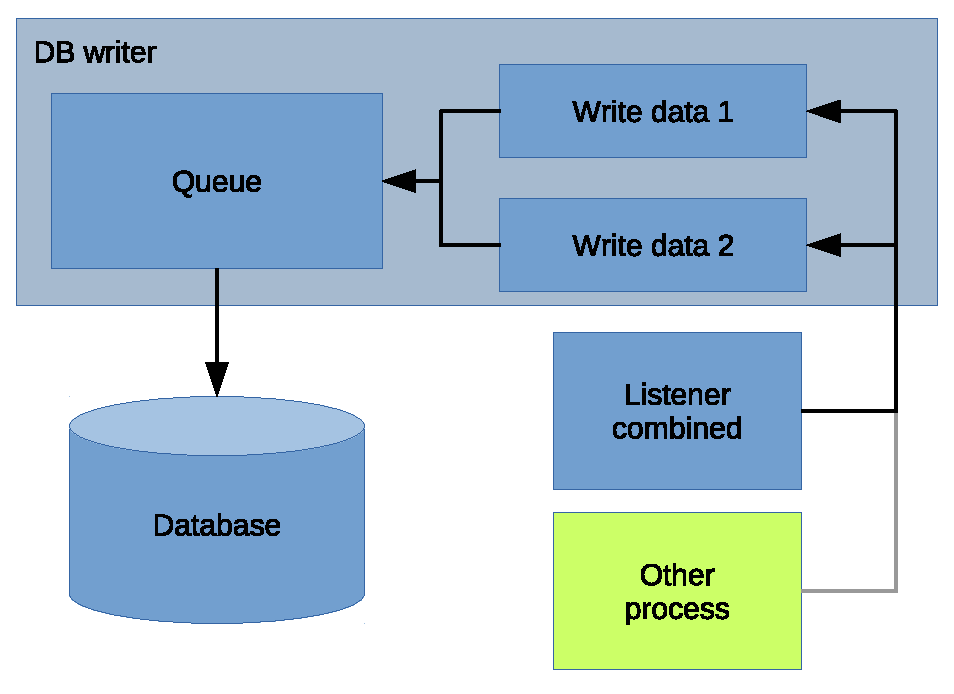
\includegraphics[width=12.64cm]{images/dbWriter.eps}
		\caption[Database writer]{Visualization of the database writer. By calling the ''write data'' methods, SQL statements are created, that are added to a queue and added to the database by a separate process. By this construction the writing process is not blocking and writing to the disk can be efficient as it only happens if a lot of write statements are executed or the queue is empty.}
		\label{fig:DBwriter}
	\end{figure}
	
	\begin{table}[H]
		
		\centering
		\begin{tabular}{|l|l|}
			\hline 
			Method & Arguments \\ 
			\hline \hline
			\begin{pbox}{6.0cm}{\vspace{.2\baselineskip}
					addIMUData(acceleration, orientation, rotation)
					\vspace{.3\baselineskip}} \end{pbox}&\begin{pbox}{6.0cm}{\vspace{.2\baselineskip}
					[\textbf{float} accX, \textbf{float} accY, \textbf{float} accZ],
					[\textbf{float} orX, \textbf{float} orY, \textbf{float} orZ],
					[\textbf{float} rotX, \textbf{float} rotY, \textbf{float} rotZ]
					\vspace{.3\baselineskip}} \end{pbox}\\ 
			\hline 
			\begin{pbox}{6.0cm}{\vspace{.2\baselineskip}
					addGPSData(longitude, latitude)
					\vspace{.3\baselineskip}} \end{pbox}&\begin{pbox}{6.0cm}{\vspace{.2\baselineskip}
					\textbf{float} longitude, \textbf{float} latitude
					\vspace{.3\baselineskip}} \end{pbox}\\ 
			\hline 
			\begin{pbox}{6.0cm}{\vspace{.2\baselineskip}
					addCommand(commandType, value=None)
					\vspace{.3\baselineskip}}
			\end{pbox}&
			\begin{pbox}{6.0cm}{\vspace{.2\baselineskip}
					\textbf{str} type, \textbf{None} or [\textbf{float} min, \textbf{float} max] 
					\vspace{.3\baselineskip}}
			\end{pbox}\\ 
			\hline 
			\begin{pbox}{6.0cm}{\vspace{.2\baselineskip}
					addSpeed(speed)	
					\vspace{.3\baselineskip}} 
			\end{pbox}&
			\begin{pbox}{6.0cm}{\vspace{.2\baselineskip}
					\textbf{float} speed
					\vspace{.3\baselineskip}}
			\end{pbox}\\ 
			\hline 
			\begin{pbox}{6.0cm}{\vspace{.2\baselineskip}
					addSteeringAngle(angle)	
					\vspace{.3\baselineskip}} 
			\end{pbox}&
			\begin{pbox}{6.0cm}{\vspace{.2\baselineskip}
					\textbf{float} angle
					\vspace{.3\baselineskip}}
			\end{pbox}\\ 
			\hline 
			\begin{pbox}{6.0cm}{\vspace{.2\baselineskip}
					addObstData(obstacles)
					\vspace{.3\baselineskip}} 
			\end{pbox}&
			\begin{pbox}{6.0cm}{\vspace{.2\baselineskip}
					[(\textbf{float} $xL_1$, \textbf{float} $xR_1$, \textbf{float} $z_1$),\\ (\textbf{float} $xL_2$, \textbf{float} $xR_2$, \textbf{float} $z_2$),\\  \dots, \\(\textbf{float} $xL_n$, \textbf{float} $xR_n$, \textbf{float} $z_n$)]
					\vspace{.3\baselineskip}}
			\end{pbox}\\ 
			\hline  
		\end{tabular} 
	\caption{Implemented methods for ''DB writer''} \label{tab:dbWriter}
		
	\end{table}
	
	\begin{figure}[H]
		\centering
		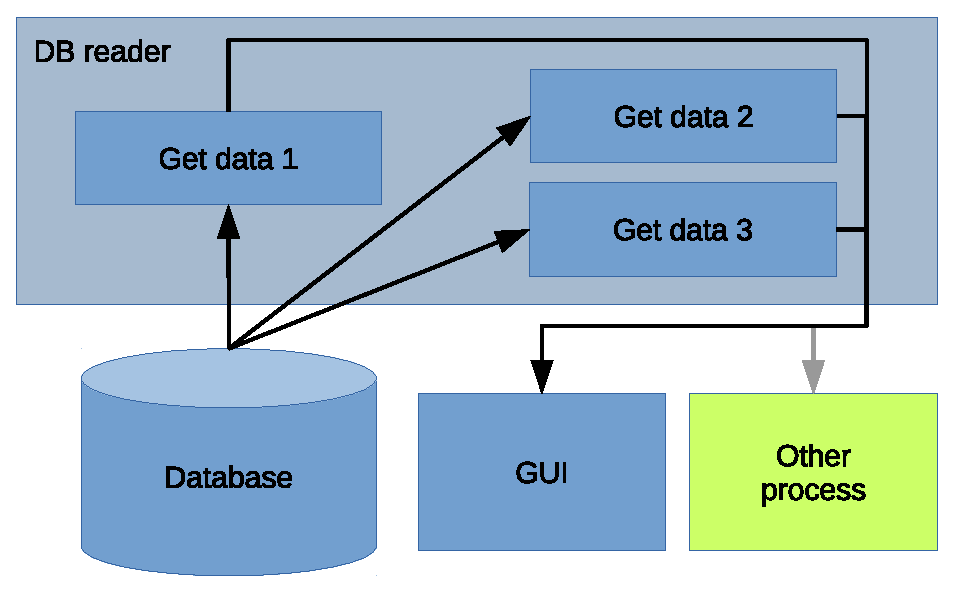
\includegraphics[width=12.64cm]{images/dbReader.eps}
		\caption[Database reader]{Visualization of the database reader. The scheme is simplified.}
		\label{fig:DBreader}
	\end{figure}
	\begin{table}[H]
		\centering
		\begin{tabular}{|l|l|}
			\hline 
			Method & Return values \\ 
			\hline \hline
			\begin{pbox}{6.0cm}{\vspace{.2\baselineskip}
					getSpeed()
					\vspace{.3\baselineskip}} \end{pbox}&\begin{pbox}{6.0cm}{\vspace{.2\baselineskip}
					[\textbf{float} $datum_1$, \dots, \textbf{float} $datum_n$], [\textbf{float} $speed_1$, \dots, \textbf{float} $speed_n$]
					\vspace{.3\baselineskip}} \end{pbox}\\ 
			\hline 
			\begin{pbox}{6.0cm}{\vspace{.2\baselineskip}
					getSteeringAngle()
					\vspace{.3\baselineskip}} \end{pbox}&\begin{pbox}{6.0cm}{\vspace{.2\baselineskip}
					[\textbf{float} $datum_1$, \dots, \textbf{float} $datum_n$], [\textbf{float} $angle_1$, \dots, \textbf{float} $angle_n$]
						\vspace{.3\baselineskip}} \end{pbox}\\ 
			\hline 
			\begin{pbox}{6.0cm}{\vspace{.2\baselineskip}
					getImuData()
					\vspace{.3\baselineskip}}
			\end{pbox}&
			\begin{pbox}{6.7cm}{\vspace{.2\baselineskip}
					[\textbf{float} $datum_1$, \dots, \textbf{float} $datum_n$],\newline
					[\textbf{float} $angVelX_1$, \dots, \textbf{float} $angVelX_n$],
					[\textbf{float} $angVelY_1$, \dots, \textbf{float} $angVelY_n$],
					[\textbf{float} $angVelZ_1$, \dots, \textbf{float} $angVelZ_n$],
					[\textbf{float} $orientX_1$, \dots, \textbf{float} $orientX_n$],
					[\textbf{float} $orientY_1$, \dots, \textbf{float} $orientY_n$],
					[\textbf{float} $orientZ_1$, \dots, \textbf{float} $orientZ_n$],
					[\textbf{float} $linAccX_1$, \dots, \textbf{float} $linAccX_n$],
					[\textbf{float} $linAccY_1$, \dots, \textbf{float} $linAccY_n$],
					[\textbf{float} $linAccZ_1$, \dots, \textbf{float} $linAccZ_n$]
					\vspace{.3\baselineskip}}\end{pbox}\\ 
			\hline 
			\begin{pbox}{6.0cm}{\vspace{.2\baselineskip}
					getCommands()
					\vspace{.3\baselineskip}} 
			\end{pbox}&
			\begin{pbox}{10.5cm}{\vspace{.2\baselineskip}
					[\textbf{float} $datum_1$, \dots, \textbf{float} $datum_n$],
					[\textbf{str} $type_1$], \dots, \textbf{str} $type_n$],\newline
					[\textbf{None} or \textbf{float list} $value_1$, \dots, \textbf{None} or \textbf{float list} $value_n$]
					\vspace{.3\baselineskip}}
			\end{pbox}\\ 
			\hline 
			\begin{pbox}{6.0cm}{\vspace{.2\baselineskip}
					getGps()
					\vspace{.3\baselineskip}} 
			\end{pbox}&
			\begin{pbox}{6.7cm}{\vspace{.2\baselineskip}
					[\textbf{float} $datum_1$, \dots, \textbf{float} $datum_n$],\newline
					[\textbf{float} $longitude_1$, \dots, \textbf{float} $longitude_n$],
					[\textbf{float} $latitude_1$, \dots, \textbf{float} $latitude_n$],
					\vspace{.3\baselineskip}}
			\end{pbox}\\ 
			\hline 
		\end{tabular}
	\caption{Implemented methods for ''DB reader''} \label{tab:dbReader} 
	\end{table}
	

\chapter{Communication}
	\label{sec:communication}
	To keep the system as flexible as possible, it is import to keep the communication independent from the underlying operating system. ROS already provides a strong communication tool but offers only good support on Linux, bad support on Windows and no support for Android. With the python built in networking packages it is possible to create a communication system that suits our purposes best.

	An overview over the communication mechanism is given in figure \ref{fig:communication}. The ''Communicator'' class in ''communicator.py'' implements both ends of the inter network communication. On the bike it is run as server and on the mobile device as client. The bike and the mobile device have to be in the same wireless network. It is possible to run the bike as 2.4 GHz hotspot and to connect the bike to it. Then the GUI can be connected to the server. Figure \ref{fig:sendMsg} shows the process of sending two different messages. The messages are transmitted using the TCP. This ensures that the messages are received. A serial number and a timestamp is added to prevent the reuse of old messages. This not yet useful, as the clocks of the bike and mobile device are not synced, but allows an easier cryptographic extension. To achieve a secure connection, only a cryptographic procedure must be added to ''Pack Msg'' and to ''Unpack Msg''.
	
	The sensor data is not sent to the GUI by default. The GUI is requesting the data, that shall be displayed. That way data that is not displayed can be excluded. The frequencies in which the data is requested can be set at the GUI, while it is running. The "Refresher" class in "communicator.py" periodically adds request messages to the priority queue. It uses a sleep command to wait the specified time. This can cause a problem if the time is set to a very high value by accident. Then this time will be waited before the higher frequency is used. It is visualized in figure \ref{fig:refresher}. Currently all displayable data is updated all the time, but the system is designed to support pausing it. In the case that the traffic induces costs, the not displayed data should not be updated. The messages are sent with different priorities (see table \ref{tab:prio}) to guarantee that certain commands are received quickly. The currently supported message types are shown in table \ref{tab:messageTypes}.
	\begin{figure}
		\centering
		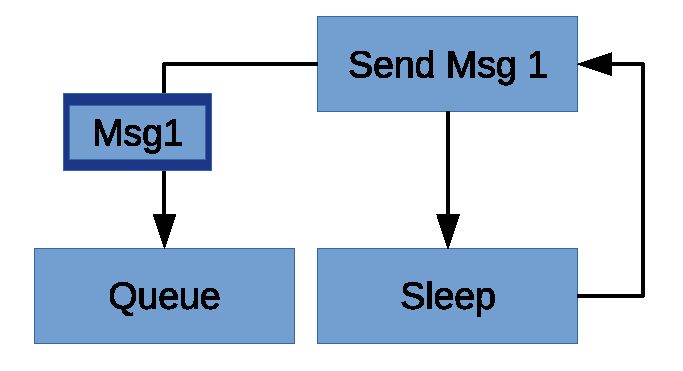
\includegraphics[width=8cm]{images/refresher.eps}
		\caption{Refresher} \label{fig:refresher}
	\end{figure}
	
	
	\begin{table}
		
		\begin{tabular}{|l|l|}
			\hline 
			Priority & Description \\ 
			\hline \hline
			TOP & 
			\begin{pbox}{11.0cm}{\vspace{.2\baselineskip}
					Highest priority will always be sent first. Currently only used for STOP messages.
					\vspace{.3\baselineskip}}
			\end{pbox}\\
			\hline 
			HIGH &
			\begin{pbox}{11.0cm}{\vspace{.2\baselineskip}
					Currently only used for SETTARGETS messages.
					\vspace{.3\baselineskip}}
			\end{pbox}\\ 
			\hline 
			NORMAL &
			\begin{pbox}{11.0cm}{\vspace{.2\baselineskip}
					Used for almost any message.
					\vspace{.3\baselineskip}}
			\end{pbox}\\
			\hline 
			LOW &
			\begin{pbox}{11.0cm}{\vspace{.2\baselineskip}
					Currently not used but might be used to transmit the video stream, if the network is overloaded.
					\vspace{.3\baselineskip}}
			\end{pbox}\\
			\hline 
		\end{tabular}
		\caption{Priorities} \label{tab:prio}		
	\end{table}

	\begin{figure}[H]
		\centering
		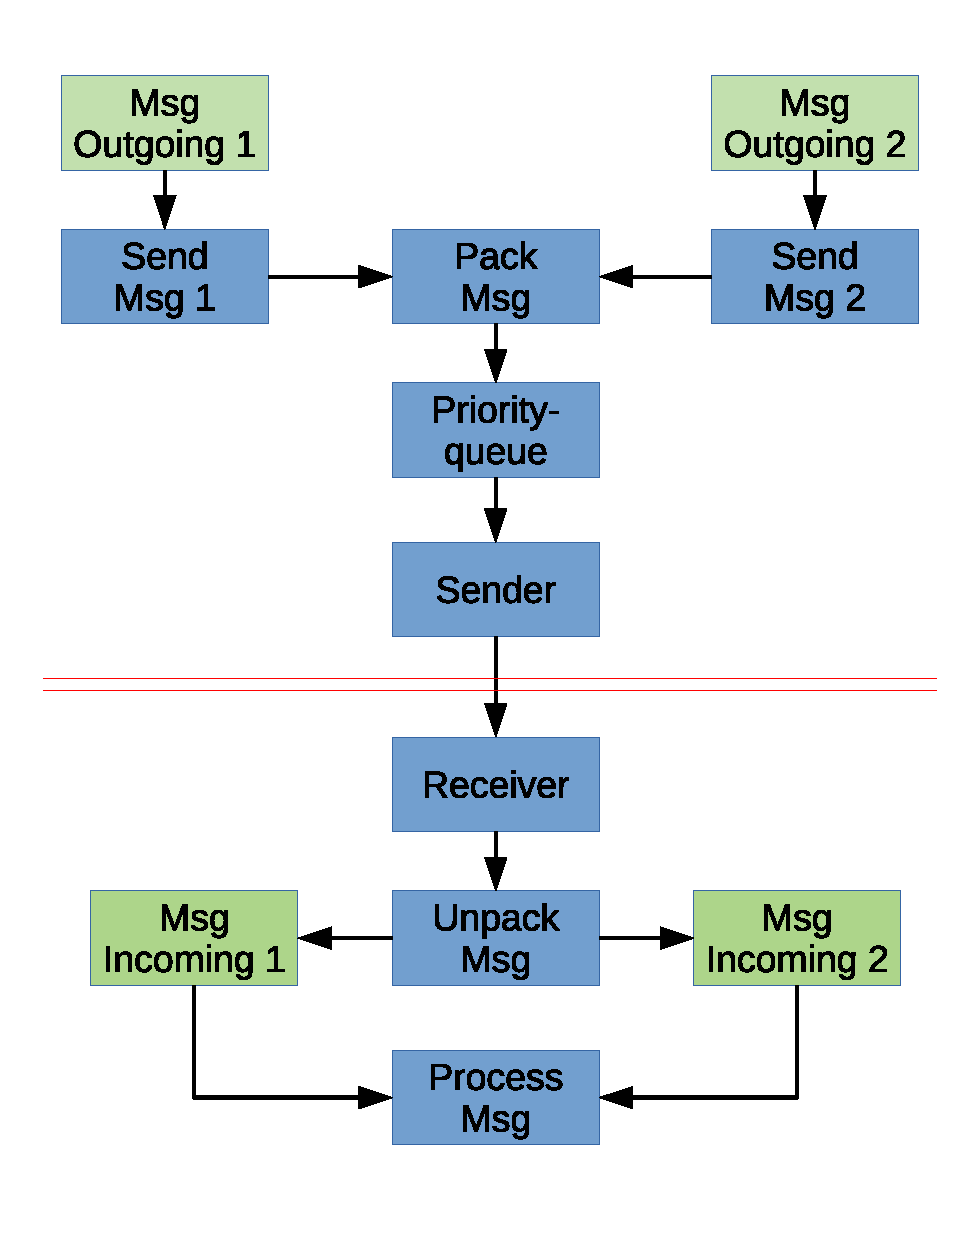
\includegraphics[width=10cm]{images/sendMsg.eps}
		\caption{Sending of two different messages. See table \ref{tab:sendMsg}}
		\label{fig:sendMsg}
	\end{figure}

	\begin{table}
		\centering
		
		\begin{tabular}{|l|l|}
			\hline
			Send Msg & \begin{pbox}{11.0cm}{\vspace{.2\baselineskip}
					Fetches important data from the system, adds a priority and forwards the message to ''Pack Msg''
					\vspace{.3\baselineskip}} 
			\end{pbox}\\
			\hline 
			Pack Msg & 
			\begin{pbox}{11.0cm}{\vspace{.2\baselineskip}
				Adds a timestamp, a serial number and a number encoding the message type. The it uses pickle to serialize the data
				\vspace{.3\baselineskip}} 
		\end{pbox}\\
			\hline
			Sender &
			\begin{pbox}{11.0cm}{\vspace{.2\baselineskip}
				Locks until the priority contains an element, then sends it to the corresponding ''Receiver''. More then one message may be sent at once, based on the usage uf TCP.\vspace{.3\baselineskip}}
			\end{pbox}\\
			\hline
			Receiver &
			\begin{pbox}{11.0cm}{\vspace{.2\baselineskip}
				Locks until data is received, then splits it to packed messages. \vspace{.3\baselineskip}}
			\end{pbox}\\
			\hline
			Unpack Msg &
			\begin{pbox}{11.0cm}{\vspace{.2\baselineskip}
				Unpickles the message and checks if it is to old or the sequence number was already used. In case of a failure (e.g. a broken message) the returned message type is \textbf{False}.
				\vspace{.3\baselineskip}}
			\end{pbox}\\
			\hline
			Process Msg &
			\begin{pbox}{11.0cm}{\vspace{.2\baselineskip}
				Checks for the message type and initiates, according to it, the following reaction.
				\vspace{.3\baselineskip}}
			\end{pbox}\\
			\hline
		\end{tabular}
	\caption{Short description of the methods involved in the sending process.
		See figure \ref{fig:sendMsg}}
	\label{tab:sendMsg}
	\end{table}

	\begin{figure}[H]
		\centering
		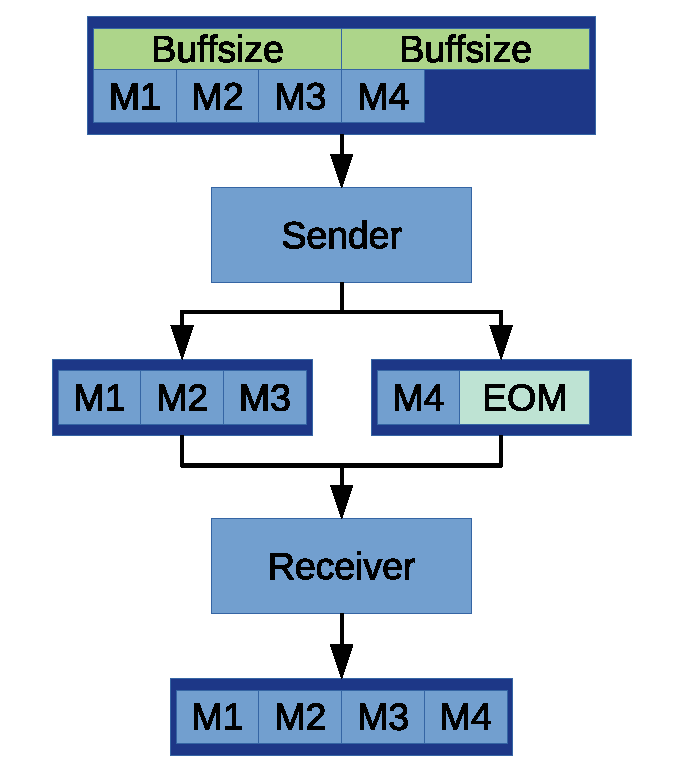
\includegraphics[width=7.5cm]{images/sendSingleMsg.eps}
		\caption[Send a single message]{Process of sending a single message. If its size exceeds Buffsize, it is split into parts of the length Buffsize. Before splitting, a ''End Of Message' string is added at the end of the message. If this string is sent through the network (which is very unlikely), the message containing it will be corrupted.}
	\end{figure}
	
	\begin{figure}[H]
		\centering
		\includegraphics[width=0.8\linewidth]{images/communication2.eps}
		\caption[Communication]{Scheme of the inter process communication from the GUI up to the ROS nodes ''GUI publisher'' and ''Listener combined''. Adjacent modules are part of the biggest one. Arrows indicate the direction of the information flow. }
		\label{fig:communication}
	\end{figure}

	\begin{table}[H]
		\centering
		
		\begin{tabular}{|l|l|l|}
			\hline 
			Message type & \textbf{int} & Description \\ 
			\hline 
			DUMMY & 0 & 
			\begin{pbox}{7.0cm}{\vspace{.2\baselineskip}
					does nothing
					\vspace{.3\baselineskip}}
			\end{pbox}\\
			\hline 
			OK & 1 & 
			\begin{pbox}{7.0cm}{\vspace{.2\baselineskip}
					acknowledge the income of a certain message
					\vspace{.3\baselineskip}}
			\end{pbox}\\
			\hline 
			SHUTDOWN & 2 & 
			\begin{pbox}{7.0cm}{\vspace{.2\baselineskip}
					stop the bike as soon as possible
					\vspace{.3\baselineskip}}
			\end{pbox}\\
			\hline 
			GETSPEED & 30 & 
			\begin{pbox}{7.0cm}{\vspace{.2\baselineskip}
					requests the current speed
					\vspace{.3\baselineskip}}
			\end{pbox}\\
			\hline 
			RETURNSPEED & 31 & 
			\begin{pbox}{7.0cm}{\vspace{.2\baselineskip}
					return for GETSPEED
					\vspace{.3\baselineskip}}
			\end{pbox}\\
			\hline 
			SETTARGETSPEED & 32 & 
			\begin{pbox}{7.0cm}{\vspace{.2\baselineskip}
					sets a new target speed value
					\vspace{.3\baselineskip}}
			\end{pbox}\\
			\hline 
			GETTARGETSPEED & 33 & 
			\begin{pbox}{7.0cm}{\vspace{.2\baselineskip}
					requests the target speed value set by Control
					\vspace{.3\baselineskip}}
			\end{pbox}\\
			\hline 
			RETURNTARGETSPEED & 34 & 
			\begin{pbox}{7.0cm}{\vspace{.2\baselineskip}
					return for GETTARGETSPEED 
					\vspace{.3\baselineskip}}
			\end{pbox}\\
			\hline 
			GETTILT & 40 & 
			\begin{pbox}{7.0cm}{\vspace{.2\baselineskip}
					request the tilt level of the bike (orientationY)
					\vspace{.3\baselineskip}}
			\end{pbox}\\
			\hline 
			RETURNTILT & 41 & 
			\begin{pbox}{7.0cm}{\vspace{.2\baselineskip}
					returns for GETTILT
					\vspace{.3\baselineskip}}
			\end{pbox}\\
			\hline 
			GETOBSTACLES & 50 & 
			\begin{pbox}{7.0cm}{\vspace{.2\baselineskip}
					requests the list of detected obstacles
					\vspace{.3\baselineskip}}
			\end{pbox}\\
			\hline 
			RETURNOBSTACLES & 51 & 
			\begin{pbox}{7.0cm}{\vspace{.2\baselineskip}
					return for GETOBSTACLES
					\vspace{.3\baselineskip}}
			\end{pbox}\\
			\hline 
			GETBATTERY & 60 & 
			\begin{pbox}{7.0cm}{\vspace{.2\baselineskip}
					requests the battery state
					\vspace{.3\baselineskip}}
			\end{pbox}\\
			\hline 
			RETURNBATTERY & 61 & 
			\begin{pbox}{7.0cm}{\vspace{.2\baselineskip}
					returns the battery state
					\vspace{.3\baselineskip}}
			\end{pbox}\\
			\hline 
			WARNING & 70 & 
			\begin{pbox}{7.0cm}{\vspace{.2\baselineskip}
					sends a message to the GUI to be displayed 
					\vspace{.3\baselineskip}}
			\end{pbox}\\
			\hline 
			GETSTEERANGLE & 90 & 
			\begin{pbox}{7.0cm}{\vspace{.2\baselineskip}
					requests the current steering angle
					\vspace{.3\baselineskip}}
			\end{pbox}\\
			\hline 
			RETURNSTEERANGLE & 91 & 
			\begin{pbox}{7.0cm}{\vspace{.2\baselineskip}
					returns for GETSTEERANGLE 
					\vspace{.3\baselineskip}}
			\end{pbox}\\
			\hline 
			GETTARGETSTEERANGLE & 92 & 
			\begin{pbox}{7.0cm}{\vspace{.2\baselineskip}
					requests the value of the current target steering angle
					\vspace{.3\baselineskip}}
			\end{pbox}\\
			\hline 
			RETURNTARGETSTEERANGLE & 93 & 
			\begin{pbox}{7.0cm}{\vspace{.2\baselineskip}
					return for GETTARGETSTEERANGLE
					\vspace{.3\baselineskip}}
			\end{pbox}\\
			\hline 
			SETTARGETSTEERANGLE & 94 & 
			\begin{pbox}{7.0cm}{\vspace{.2\baselineskip}
					sets a new value for the target steering angle
					\vspace{.3\baselineskip}}
			\end{pbox}\\
			\hline 
			GETORIENTATION & 100 & 
			\begin{pbox}{7.0cm}{\vspace{.2\baselineskip}
					requests the orientation of the IMU
					\vspace{.3\baselineskip}}
			\end{pbox}\\
			\hline 
			RETURNORIENTATION & 101 & 
			\begin{pbox}{7.0cm}{\vspace{.2\baselineskip}
					return for GETORIENTATION
					\vspace{.3\baselineskip}}
			\end{pbox}\\
			\hline 
			GETCAMERAIMAGE & 110 & 
			\begin{pbox}{7.0cm}{\vspace{.2\baselineskip}
					requests the current camera image
					\vspace{.3\baselineskip}}
			\end{pbox}\\
			\hline 
			RETURNCAMERAIMAGE & 111 & 
			\begin{pbox}{7.0cm}{\vspace{.2\baselineskip}
					return fpr GETCAMERAIMAGE
					\vspace{.3\baselineskip}}
			\end{pbox}\\
			\hline 
			UPDATELIMITS & 120 & 
			\begin{pbox}{7.0cm}{\vspace{.2\baselineskip}
					sends new values for the maximum and minimum tilt angle
					\vspace{.3\baselineskip}}
			\end{pbox}\\
			\hline 
			SETTARGETS & 130 & 
			\begin{pbox}{7.0cm}{\vspace{.2\baselineskip}
					sends new values for target speed and target angle
					\vspace{.3\baselineskip}}
			\end{pbox}\\
			\hline 
		\end{tabular}
		\caption{List of supported message types. Not all types are in use. New message types can be added easily.}
		\label{tab:messageTypes}

	\end{table}
	
	The tables \ref{tab:IntVis}, \ref{tab:IntCont}, \ref{tab:IntObst} and \ref{tab:IntCore} are based on the file "Interfaces.pdf" and the content of them were provided by the groups providing the data. E.g. the content of table \ref{tab:IntObst} was provided by the obstacle detection group. All received data is expected to be of the stated types and in the specified units.
	
	\begin{table}[H]
		\centering
		\begin{tabular}{|l|l|l|}
			\hline 
			& Type & Additional information \\ 
			\hline \hline
			Target speed & \textbf{float} & km/h [0:35] \\ 
			\hline 
			Target steering angle & \textbf{float} & degree [-90:90] \\ 
			\hline 
			STOP & \textbf{bool} & Emergency stop signal for control. \\ 
			\hline 
		\end{tabular}
		\caption[Interfaces I]{Datatypes provided by the Visualization group}
		\label{tab:IntVis}
	\end{table}

	\begin{table}[H]
		\centering
		\begin{tabular}{|l|l|l|}
			\hline 
			& Type & Additional information \\ 
			\hline \hline
			Speed & \textbf{float} & km/h [0:35] \\ 
			\hline 
			Steering angle & \textbf{float} & Radiant [-100:100] \\ 
			\hline
		\end{tabular}
		\caption[Interfaces II]{Datatypes provided by the Control group}
		\label{tab:IntCont}
	\end{table}

	\begin{table}[H]
		\centering
		\begin{tabular}{|l|l|l|}
			\hline 
			& Type & Additional information \\ 
			\hline \hline
			Obstacles &
			\begin{pbox}{5.0cm}{\vspace{.2\baselineskip}
				$[(xL_1, xR_1, z_1), (xL_2, xR_2, z_2),$ \dots$,(xL_n, xR_n, z_n]$
				\vspace{.3\baselineskip}}
			\end{pbox}
			& \begin{pbox}{5.0cm}{\vspace{.2\baselineskip}
				Coordinates relative to bike in world units (m/cm)
				\vspace{.3\baselineskip}}
			\end{pbox}\\
			\hline
		\end{tabular}
		\caption[Interfaces III]{Datatypes provided by the Obstacle detection group}
		\label{tab:IntObst}	
	\end{table}
	
	\begin{table}[H]
		\centering
		\begin{tabular}{|l|l|l|}
			\hline 
			& Type & Additional information \\ 
			\hline \hline
			Orientation & \textbf{float} & values are in degrees \\ 
			\hline 
			Linear Acceleration & \textbf{float} & values are in meter per second per second $(\frac{m}{s^2})$ \\ 
			\hline 
			GPS data & \textbf{float} & Longitude and Latitude Coordinates \\ 
			\hline 
			Angular Velocity & \textbf{float} & values are in rad/s \\ 
			\hline 
		\end{tabular} 
		\caption[Interfaces IV]{Datatypes provided by the Core group}
		\label{tab:IntCore}
	\end{table}



\chapter{Student project}

\listoffigures
\listoftables
	
\end{document}          
